\documentclass[twoside]{book}

% Packages required by doxygen
\usepackage{fixltx2e}
\usepackage{calc}
\usepackage{doxygen}
\usepackage[export]{adjustbox} % also loads graphicx
\usepackage{graphicx}
\usepackage[utf8]{inputenc}
\usepackage{makeidx}
\usepackage{multicol}
\usepackage{multirow}
\PassOptionsToPackage{warn}{textcomp}
\usepackage{textcomp}
\usepackage[nointegrals]{wasysym}
\usepackage[table]{xcolor}

% Font selection
\usepackage[T1]{fontenc}
\usepackage[scaled=.90]{helvet}
\usepackage{courier}
\usepackage{amssymb}
\usepackage{sectsty}
\renewcommand{\familydefault}{\sfdefault}
\allsectionsfont{%
  \fontseries{bc}\selectfont%
  \color{darkgray}%
}
\renewcommand{\DoxyLabelFont}{%
  \fontseries{bc}\selectfont%
  \color{darkgray}%
}
\newcommand{\+}{\discretionary{\mbox{\scriptsize$\hookleftarrow$}}{}{}}

% Page & text layout
\usepackage{geometry}
\geometry{%
  a4paper,%
  top=2.5cm,%
  bottom=2.5cm,%
  left=2.5cm,%
  right=2.5cm%
}
\tolerance=750
\hfuzz=15pt
\hbadness=750
\setlength{\emergencystretch}{15pt}
\setlength{\parindent}{0cm}
\setlength{\parskip}{3ex plus 2ex minus 2ex}
\makeatletter
\renewcommand{\paragraph}{%
  \@startsection{paragraph}{4}{0ex}{-1.0ex}{1.0ex}{%
    \normalfont\normalsize\bfseries\SS@parafont%
  }%
}
\renewcommand{\subparagraph}{%
  \@startsection{subparagraph}{5}{0ex}{-1.0ex}{1.0ex}{%
    \normalfont\normalsize\bfseries\SS@subparafont%
  }%
}
\makeatother

% Headers & footers
\usepackage{fancyhdr}
\pagestyle{fancyplain}
\fancyhead[LE]{\fancyplain{}{\bfseries\thepage}}
\fancyhead[CE]{\fancyplain{}{}}
\fancyhead[RE]{\fancyplain{}{\bfseries\leftmark}}
\fancyhead[LO]{\fancyplain{}{\bfseries\rightmark}}
\fancyhead[CO]{\fancyplain{}{}}
\fancyhead[RO]{\fancyplain{}{\bfseries\thepage}}
\fancyfoot[LE]{\fancyplain{}{}}
\fancyfoot[CE]{\fancyplain{}{}}
\fancyfoot[RE]{\fancyplain{}{\bfseries\scriptsize Generated by Doxygen }}
\fancyfoot[LO]{\fancyplain{}{\bfseries\scriptsize Generated by Doxygen }}
\fancyfoot[CO]{\fancyplain{}{}}
\fancyfoot[RO]{\fancyplain{}{}}
\renewcommand{\footrulewidth}{0.4pt}
\renewcommand{\chaptermark}[1]{%
  \markboth{#1}{}%
}
\renewcommand{\sectionmark}[1]{%
  \markright{\thesection\ #1}%
}

% Indices & bibliography
\usepackage{natbib}
\usepackage[titles]{tocloft}
\setcounter{tocdepth}{3}
\setcounter{secnumdepth}{5}
\makeindex

% Custom commands
\newcommand{\clearemptydoublepage}{%
  \newpage{\pagestyle{empty}\cleardoublepage}%
}

\usepackage{caption}
\captionsetup{labelsep=space,justification=centering,font={bf},singlelinecheck=off,skip=4pt,position=top}

%===== C O N T E N T S =====

\begin{document}

% Titlepage & ToC
\pagenumbering{alph}
\begin{titlepage}
\vspace*{7cm}
\begin{center}%
{\Large My Project }\\
\vspace*{1cm}
{\large Generated by Doxygen 1.8.13}\\
\end{center}
\end{titlepage}
\clearemptydoublepage
\pagenumbering{roman}
\tableofcontents
\clearemptydoublepage
\pagenumbering{arabic}

%--- Begin generated contents ---
\chapter{Namespace Index}
\section{Packages}
Here are the packages with brief descriptions (if available)\+:\begin{DoxyCompactList}
\item\contentsline{section}{\textbf{ D\+S\+Project\+\_\+\+Universal\+\_\+} }{\pageref{namespace_d_s_project___universal__}}{}
\item\contentsline{section}{\textbf{ D\+S\+Project\+\_\+\+Universal\+\_\+.\+D\+S\+Project\+\_\+\+Universal\+\_\+\+\_\+\+Xaml\+Type\+Info} }{\pageref{namespace_d_s_project___universal___1_1_d_s_project___universal_____xaml_type_info}}{}
\item\contentsline{section}{\textbf{ D\+S\+Project\+\_\+\+Universal\+\_\+.\+View} }{\pageref{namespace_d_s_project___universal___1_1_view}}{}
\item\contentsline{section}{\textbf{ D\+S\+Project\+Universal} }{\pageref{namespace_d_s_project_universal}}{}
\item\contentsline{section}{\textbf{ D\+S\+Project\+Universal.\+Model} }{\pageref{namespace_d_s_project_universal_1_1_model}}{}
\item\contentsline{section}{\textbf{ D\+S\+Project\+Universal.\+Util} }{\pageref{namespace_d_s_project_universal_1_1_util}}{}
\end{DoxyCompactList}

\chapter{Hierarchical Index}
\section{Class Hierarchy}
This inheritance list is sorted roughly, but not completely, alphabetically\+:\begin{DoxyCompactList}
\item Application\begin{DoxyCompactList}
\item \contentsline{section}{D\+S\+Project\+\_\+\+Universal\+\_\+.\+App}{\pageref{class_d_s_project___universal___1_1_app}}{}
\item \contentsline{section}{D\+S\+Project\+\_\+\+Universal\+\_\+.\+App}{\pageref{class_d_s_project___universal___1_1_app}}{}
\item \contentsline{section}{D\+S\+Project\+\_\+\+Universal\+\_\+.\+App}{\pageref{class_d_s_project___universal___1_1_app}}{}
\item \contentsline{section}{D\+S\+Project\+\_\+\+Universal\+\_\+.\+App}{\pageref{class_d_s_project___universal___1_1_app}}{}
\end{DoxyCompactList}
\item I\+Component\+Connector\begin{DoxyCompactList}
\item \contentsline{section}{D\+S\+Project\+\_\+\+Universal\+\_\+.\+Main\+Page}{\pageref{class_d_s_project___universal___1_1_main_page}}{}
\item \contentsline{section}{D\+S\+Project\+\_\+\+Universal\+\_\+.\+View.\+Linked\+List\+Test}{\pageref{class_d_s_project___universal___1_1_view_1_1_linked_list_test}}{}
\item \contentsline{section}{D\+S\+Project\+\_\+\+Universal\+\_\+.\+View.\+Root\+Page}{\pageref{class_d_s_project___universal___1_1_view_1_1_root_page}}{}
\end{DoxyCompactList}
\item I\+Component\+Connector2\begin{DoxyCompactList}
\item \contentsline{section}{D\+S\+Project\+\_\+\+Universal\+\_\+.\+Main\+Page}{\pageref{class_d_s_project___universal___1_1_main_page}}{}
\item \contentsline{section}{D\+S\+Project\+\_\+\+Universal\+\_\+.\+View.\+Linked\+List\+Test}{\pageref{class_d_s_project___universal___1_1_view_1_1_linked_list_test}}{}
\item \contentsline{section}{D\+S\+Project\+\_\+\+Universal\+\_\+.\+View.\+Root\+Page}{\pageref{class_d_s_project___universal___1_1_view_1_1_root_page}}{}
\end{DoxyCompactList}
\item I\+Xaml\+Metadata\+Provider\begin{DoxyCompactList}
\item \contentsline{section}{D\+S\+Project\+\_\+\+Universal\+\_\+.\+App}{\pageref{class_d_s_project___universal___1_1_app}}{}
\end{DoxyCompactList}
\item \contentsline{section}{D\+S\+Project\+Universal.\+Util.\+Linked\+List$<$ T $>$}{\pageref{class_d_s_project_universal_1_1_util_1_1_linked_list}}{}
\item \contentsline{section}{D\+S\+Project\+Universal.\+Util.\+Linked\+List$<$ D\+S\+Project\+Universal.\+Model.\+Service $>$}{\pageref{class_d_s_project_universal_1_1_util_1_1_linked_list}}{}
\item \contentsline{section}{D\+S\+Project\+Universal.\+Util.\+Linked\+List$<$ D\+S\+Project\+Universal.\+Model.\+Sub\+Service $>$}{\pageref{class_d_s_project_universal_1_1_util_1_1_linked_list}}{}
\item \contentsline{section}{D\+S\+Project\+Universal.\+Util.\+Linked\+List$<$ D\+S\+Project\+Universal.\+Model.\+Super\+Service $>$}{\pageref{class_d_s_project_universal_1_1_util_1_1_linked_list}}{}
\item \contentsline{section}{D\+S\+Project\+Universal.\+Util.\+Node$<$ T $>$}{\pageref{class_d_s_project_universal_1_1_util_1_1_node}}{}
\item Page\begin{DoxyCompactList}
\item \contentsline{section}{D\+S\+Project\+\_\+\+Universal\+\_\+.\+Main\+Page}{\pageref{class_d_s_project___universal___1_1_main_page}}{}
\item \contentsline{section}{D\+S\+Project\+\_\+\+Universal\+\_\+.\+Main\+Page}{\pageref{class_d_s_project___universal___1_1_main_page}}{}
\item \contentsline{section}{D\+S\+Project\+\_\+\+Universal\+\_\+.\+Main\+Page}{\pageref{class_d_s_project___universal___1_1_main_page}}{}
\item \contentsline{section}{D\+S\+Project\+\_\+\+Universal\+\_\+.\+View.\+Linked\+List\+Test}{\pageref{class_d_s_project___universal___1_1_view_1_1_linked_list_test}}{}
\item \contentsline{section}{D\+S\+Project\+\_\+\+Universal\+\_\+.\+View.\+Linked\+List\+Test}{\pageref{class_d_s_project___universal___1_1_view_1_1_linked_list_test}}{}
\item \contentsline{section}{D\+S\+Project\+\_\+\+Universal\+\_\+.\+View.\+Linked\+List\+Test}{\pageref{class_d_s_project___universal___1_1_view_1_1_linked_list_test}}{}
\item \contentsline{section}{D\+S\+Project\+\_\+\+Universal\+\_\+.\+View.\+Root\+Page}{\pageref{class_d_s_project___universal___1_1_view_1_1_root_page}}{}
\item \contentsline{section}{D\+S\+Project\+\_\+\+Universal\+\_\+.\+View.\+Root\+Page}{\pageref{class_d_s_project___universal___1_1_view_1_1_root_page}}{}
\item \contentsline{section}{D\+S\+Project\+\_\+\+Universal\+\_\+.\+View.\+Root\+Page}{\pageref{class_d_s_project___universal___1_1_view_1_1_root_page}}{}
\end{DoxyCompactList}
\item Page\begin{DoxyCompactList}
\item \contentsline{section}{D\+S\+Project\+\_\+\+Universal\+\_\+.\+Main\+Page}{\pageref{class_d_s_project___universal___1_1_main_page}}{}
\item \contentsline{section}{D\+S\+Project\+\_\+\+Universal\+\_\+.\+View.\+Linked\+List\+Test}{\pageref{class_d_s_project___universal___1_1_view_1_1_linked_list_test}}{}
\end{DoxyCompactList}
\item \contentsline{section}{D\+S\+Project\+Universal.\+Model.\+Service\+Pool}{\pageref{class_d_s_project_universal_1_1_model_1_1_service_pool}}{}
\item \contentsline{section}{D\+S\+Project\+Universal.\+Model.\+Sub\+Service\+Pool}{\pageref{class_d_s_project_universal_1_1_model_1_1_sub_service_pool}}{}
\item \contentsline{section}{D\+S\+Project\+Universal.\+Model.\+Super\+Service}{\pageref{class_d_s_project_universal_1_1_model_1_1_super_service}}{}
\begin{DoxyCompactList}
\item \contentsline{section}{D\+S\+Project\+Universal.\+Model.\+Service}{\pageref{class_d_s_project_universal_1_1_model_1_1_service}}{}
\item \contentsline{section}{D\+S\+Project\+Universal.\+Model.\+Sub\+Service}{\pageref{class_d_s_project_universal_1_1_model_1_1_sub_service}}{}
\end{DoxyCompactList}
\end{DoxyCompactList}

\chapter{Class Index}
\section{Class List}
Here are the classes, structs, unions and interfaces with brief descriptions\+:\begin{DoxyCompactList}
\item\contentsline{section}{\textbf{ D\+S\+Project\+\_\+\+Universal\+\_\+.\+App} \\*Provides application-\/specific behavior to supplement the default Application class. }{\pageref{class_d_s_project___universal___1_1_app}}{}
\item\contentsline{section}{\textbf{ D\+S\+Project\+Universal.\+Util.\+Linked\+List$<$ T $>$} \\*A Linked list structure to store data}{\pageref{class_d_s_project_universal_1_1_util_1_1_linked_list}}{}
\item\contentsline{section}{\textbf{ D\+S\+Project\+\_\+\+Universal\+\_\+.\+View.\+Linked\+List\+Test} \\*An empty page that can be used on its own or navigated to within a Frame. }{\pageref{class_d_s_project___universal___1_1_view_1_1_linked_list_test}}{}
\item\contentsline{section}{\textbf{ D\+S\+Project\+\_\+\+Universal\+\_\+.\+Main\+Page} \\*An empty page that can be used on its own or navigated to within a Frame. }{\pageref{class_d_s_project___universal___1_1_main_page}}{}
\item\contentsline{section}{\textbf{ D\+S\+Project\+Universal.\+Util.\+Node$<$ T $>$} \\*Class of objects representing nodes of a linked list}{\pageref{class_d_s_project_universal_1_1_util_1_1_node}}{}
\item\contentsline{section}{\textbf{ D\+S\+Project\+\_\+\+Universal\+\_\+.\+View.\+Root\+Page} \\*An empty page that can be used on its own or navigated to within a Frame. }{\pageref{class_d_s_project___universal___1_1_view_1_1_root_page}}{}
\item\contentsline{section}{\textbf{ D\+S\+Project\+Universal.\+Model.\+Service} }{\pageref{class_d_s_project_universal_1_1_model_1_1_service}}{}
\item\contentsline{section}{\textbf{ D\+S\+Project\+Universal.\+Model.\+Service\+Pool} \\*A place to store all active services}{\pageref{class_d_s_project_universal_1_1_model_1_1_service_pool}}{}
\item\contentsline{section}{\textbf{ D\+S\+Project\+Universal.\+Model.\+Sub\+Service} }{\pageref{class_d_s_project_universal_1_1_model_1_1_sub_service}}{}
\item\contentsline{section}{\textbf{ D\+S\+Project\+Universal.\+Model.\+Sub\+Service\+Pool} \\*A place to store all active subservices}{\pageref{class_d_s_project_universal_1_1_model_1_1_sub_service_pool}}{}
\item\contentsline{section}{\textbf{ D\+S\+Project\+Universal.\+Model.\+Super\+Service} \\*An abstract represents services and subservices}{\pageref{class_d_s_project_universal_1_1_model_1_1_super_service}}{}
\end{DoxyCompactList}

\chapter{Namespace Documentation}
\section{D\+S\+Project\+\_\+\+Universal\+\_\+ Namespace Reference}
\label{namespace_d_s_project___universal__}\index{D\+S\+Project\+\_\+\+Universal\+\_\+@{D\+S\+Project\+\_\+\+Universal\+\_\+}}
\subsection*{Namespaces}
\begin{DoxyCompactItemize}
\end{DoxyCompactItemize}
\subsection*{Classes}
\begin{DoxyCompactItemize}
\item 
class \textbf{ App}
\begin{DoxyCompactList}\small\item\em Provides application-\/specific behavior to supplement the default Application class. \end{DoxyCompactList}\item 
class \textbf{ Main\+Page}
\begin{DoxyCompactList}\small\item\em An empty page that can be used on its own or navigated to within a Frame. \end{DoxyCompactList}\item 
class {\bfseries Program}
\begin{DoxyCompactList}\small\item\em Program class \end{DoxyCompactList}\end{DoxyCompactItemize}

\section{D\+S\+Project\+\_\+\+Universal\+\_\+.\+D\+S\+Project\+\_\+\+Universal\+\_\+\+\_\+\+Xaml\+Type\+Info Namespace Reference}
\label{namespace_d_s_project___universal___1_1_d_s_project___universal_____xaml_type_info}\index{D\+S\+Project\+\_\+\+Universal\+\_\+.\+D\+S\+Project\+\_\+\+Universal\+\_\+\+\_\+\+Xaml\+Type\+Info@{D\+S\+Project\+\_\+\+Universal\+\_\+.\+D\+S\+Project\+\_\+\+Universal\+\_\+\+\_\+\+Xaml\+Type\+Info}}
\subsection*{Classes}
\begin{DoxyCompactItemize}
\item 
class {\bfseries Xaml\+Member}
\item 
class {\bfseries Xaml\+System\+Base\+Type}
\item 
class {\bfseries Xaml\+Type\+Info\+Provider}
\item 
class {\bfseries Xaml\+User\+Type}
\end{DoxyCompactItemize}

\section{D\+S\+Project\+\_\+\+Universal\+\_\+.\+View Namespace Reference}
\label{namespace_d_s_project___universal___1_1_view}\index{D\+S\+Project\+\_\+\+Universal\+\_\+.\+View@{D\+S\+Project\+\_\+\+Universal\+\_\+.\+View}}
\subsection*{Classes}
\begin{DoxyCompactItemize}
\item 
class \textbf{ Linked\+List\+Test}
\begin{DoxyCompactList}\small\item\em An empty page that can be used on its own or navigated to within a Frame. \end{DoxyCompactList}\item 
class \textbf{ Root\+Page}
\begin{DoxyCompactList}\small\item\em An empty page that can be used on its own or navigated to within a Frame. \end{DoxyCompactList}\end{DoxyCompactItemize}

\section{D\+S\+Project\+Universal Namespace Reference}
\label{namespace_d_s_project_universal}\index{D\+S\+Project\+Universal@{D\+S\+Project\+Universal}}
\subsection*{Namespaces}
\begin{DoxyCompactItemize}
\end{DoxyCompactItemize}

\section{D\+S\+Project\+Universal.\+Model Namespace Reference}
\label{namespace_d_s_project_universal_1_1_model}\index{D\+S\+Project\+Universal.\+Model@{D\+S\+Project\+Universal.\+Model}}
\subsection*{Classes}
\begin{DoxyCompactItemize}
\item 
class \textbf{ Service}
\item 
class \textbf{ Service\+Pool}
\begin{DoxyCompactList}\small\item\em A place to store all active services\end{DoxyCompactList}\item 
class \textbf{ Sub\+Service}
\item 
class \textbf{ Sub\+Service\+Pool}
\begin{DoxyCompactList}\small\item\em A place to store all active subservices\end{DoxyCompactList}\item 
class \textbf{ Super\+Service}
\begin{DoxyCompactList}\small\item\em An abstract represents services and subservices\end{DoxyCompactList}\end{DoxyCompactItemize}

\section{D\+S\+Project\+Universal.\+Util Namespace Reference}
\label{namespace_d_s_project_universal_1_1_util}\index{D\+S\+Project\+Universal.\+Util@{D\+S\+Project\+Universal.\+Util}}
\subsection*{Classes}
\begin{DoxyCompactItemize}
\item 
class \textbf{ Linked\+List}
\begin{DoxyCompactList}\small\item\em A Linked list structure to store data\end{DoxyCompactList}\item 
class \textbf{ Node}
\begin{DoxyCompactList}\small\item\em Class of objects representing nodes of a linked list\end{DoxyCompactList}\end{DoxyCompactItemize}

\chapter{Class Documentation}
\section{D\+S\+Project\+\_\+\+Universal\+\_\+.\+App Class Reference}
\label{class_d_s_project___universal___1_1_app}\index{D\+S\+Project\+\_\+\+Universal\+\_\+.\+App@{D\+S\+Project\+\_\+\+Universal\+\_\+.\+App}}


Provides application-\/specific behavior to supplement the default Application class.  


Inheritance diagram for D\+S\+Project\+\_\+\+Universal\+\_\+.\+App\+:\begin{figure}[H]
\begin{center}
\leavevmode
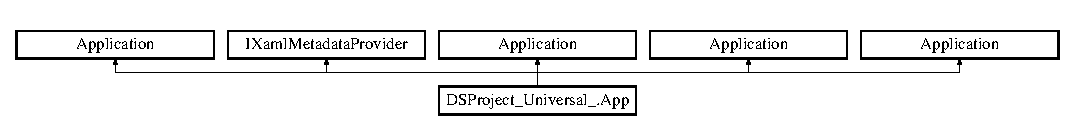
\includegraphics[height=1.309942cm]{class_d_s_project___universal___1_1_app}
\end{center}
\end{figure}
\subsection*{Public Member Functions}
\begin{DoxyCompactItemize}
\item 
\textbf{ App} ()
\begin{DoxyCompactList}\small\item\em Initializes the singleton application object. This is the first line of authored code executed, and as such is the logical equivalent of main() or Win\+Main(). \end{DoxyCompactList}\item 
void \textbf{ Initialize\+Component} ()
\begin{DoxyCompactList}\small\item\em \doxyref{Initialize\+Component()}{p.}{class_d_s_project___universal___1_1_app_afc1a80cc5544825bfcd164df897e90cc} \end{DoxyCompactList}\item 
global\+::\+Windows.\+U\+I.\+Xaml.\+Markup.\+I\+Xaml\+Type \textbf{ Get\+Xaml\+Type} (global\+::\+System.\+Type type)
\begin{DoxyCompactList}\small\item\em Get\+Xaml\+Type(\+Type) \end{DoxyCompactList}\item 
global\+::\+Windows.\+U\+I.\+Xaml.\+Markup.\+I\+Xaml\+Type \textbf{ Get\+Xaml\+Type} (string full\+Name)
\begin{DoxyCompactList}\small\item\em Get\+Xaml\+Type(\+String) \end{DoxyCompactList}\item 
global\+::\+Windows.\+U\+I.\+Xaml.\+Markup.\+Xmlns\+Definition [$\,$] \textbf{ Get\+Xmlns\+Definitions} ()
\begin{DoxyCompactList}\small\item\em \doxyref{Get\+Xmlns\+Definitions()}{p.}{class_d_s_project___universal___1_1_app_a960b100e72a7bdeb7c63b42a2dae6d83} \end{DoxyCompactList}\item 
void \textbf{ Initialize\+Component} ()
\begin{DoxyCompactList}\small\item\em \doxyref{Initialize\+Component()}{p.}{class_d_s_project___universal___1_1_app_afc1a80cc5544825bfcd164df897e90cc} \end{DoxyCompactList}\end{DoxyCompactItemize}
\subsection*{Protected Member Functions}
\begin{DoxyCompactItemize}
\item 
override void \textbf{ On\+Launched} (Launch\+Activated\+Event\+Args e)
\begin{DoxyCompactList}\small\item\em Invoked when the application is launched normally by the end user. Other entry points will be used such as when the application is launched to open a specific file. \end{DoxyCompactList}\end{DoxyCompactItemize}
\subsection*{Properties}
\begin{DoxyCompactItemize}
\item 
\mbox{\label{class_d_s_project___universal___1_1_app_a23ba48be381cdbab991e9eddaae0d11d}} 
static \textbf{ Service\+Pool} {\bfseries Service\+Pool}\hspace{0.3cm}{\ttfamily  [get]}
\item 
\mbox{\label{class_d_s_project___universal___1_1_app_a4fe355ee907b61b09a57a6199ebfbad4}} 
static \textbf{ Sub\+Service\+Pool} {\bfseries Sub\+Service\+Pool}\hspace{0.3cm}{\ttfamily  [get]}
\end{DoxyCompactItemize}


\subsection{Detailed Description}
Provides application-\/specific behavior to supplement the default Application class. 



\subsection{Constructor \& Destructor Documentation}
\mbox{\label{class_d_s_project___universal___1_1_app_ac2c8b62a78076c9eddd8fb48a035fa36}} 
\index{D\+S\+Project\+\_\+\+Universal\+\_\+\+::\+App@{D\+S\+Project\+\_\+\+Universal\+\_\+\+::\+App}!App@{App}}
\index{App@{App}!D\+S\+Project\+\_\+\+Universal\+\_\+\+::\+App@{D\+S\+Project\+\_\+\+Universal\+\_\+\+::\+App}}
\subsubsection{App()}
{\footnotesize\ttfamily D\+S\+Project\+\_\+\+Universal\+\_\+.\+App.\+App (\begin{DoxyParamCaption}{ }\end{DoxyParamCaption})}



Initializes the singleton application object. This is the first line of authored code executed, and as such is the logical equivalent of main() or Win\+Main(). 



\subsection{Member Function Documentation}
\mbox{\label{class_d_s_project___universal___1_1_app_aceac8acc372e767a1cb364598ec4a416}} 
\index{D\+S\+Project\+\_\+\+Universal\+\_\+\+::\+App@{D\+S\+Project\+\_\+\+Universal\+\_\+\+::\+App}!Get\+Xaml\+Type@{Get\+Xaml\+Type}}
\index{Get\+Xaml\+Type@{Get\+Xaml\+Type}!D\+S\+Project\+\_\+\+Universal\+\_\+\+::\+App@{D\+S\+Project\+\_\+\+Universal\+\_\+\+::\+App}}
\subsubsection{Get\+Xaml\+Type()\hspace{0.1cm}{\footnotesize\ttfamily [1/2]}}
{\footnotesize\ttfamily global.\+Windows.\+U\+I.\+Xaml.\+Markup.\+I\+Xaml\+Type D\+S\+Project\+\_\+\+Universal\+\_\+.\+App.\+Get\+Xaml\+Type (\begin{DoxyParamCaption}\item[{global\+::\+System.\+Type}]{type }\end{DoxyParamCaption})}



Get\+Xaml\+Type(\+Type) 

\mbox{\label{class_d_s_project___universal___1_1_app_a9e05eb746093bc21be27b5e71e91b2a7}} 
\index{D\+S\+Project\+\_\+\+Universal\+\_\+\+::\+App@{D\+S\+Project\+\_\+\+Universal\+\_\+\+::\+App}!Get\+Xaml\+Type@{Get\+Xaml\+Type}}
\index{Get\+Xaml\+Type@{Get\+Xaml\+Type}!D\+S\+Project\+\_\+\+Universal\+\_\+\+::\+App@{D\+S\+Project\+\_\+\+Universal\+\_\+\+::\+App}}
\subsubsection{Get\+Xaml\+Type()\hspace{0.1cm}{\footnotesize\ttfamily [2/2]}}
{\footnotesize\ttfamily global.\+Windows.\+U\+I.\+Xaml.\+Markup.\+I\+Xaml\+Type D\+S\+Project\+\_\+\+Universal\+\_\+.\+App.\+Get\+Xaml\+Type (\begin{DoxyParamCaption}\item[{string}]{full\+Name }\end{DoxyParamCaption})}



Get\+Xaml\+Type(\+String) 

\mbox{\label{class_d_s_project___universal___1_1_app_a960b100e72a7bdeb7c63b42a2dae6d83}} 
\index{D\+S\+Project\+\_\+\+Universal\+\_\+\+::\+App@{D\+S\+Project\+\_\+\+Universal\+\_\+\+::\+App}!Get\+Xmlns\+Definitions@{Get\+Xmlns\+Definitions}}
\index{Get\+Xmlns\+Definitions@{Get\+Xmlns\+Definitions}!D\+S\+Project\+\_\+\+Universal\+\_\+\+::\+App@{D\+S\+Project\+\_\+\+Universal\+\_\+\+::\+App}}
\subsubsection{Get\+Xmlns\+Definitions()}
{\footnotesize\ttfamily global.\+Windows.\+U\+I.\+Xaml.\+Markup.\+Xmlns\+Definition [$\,$] D\+S\+Project\+\_\+\+Universal\+\_\+.\+App.\+Get\+Xmlns\+Definitions (\begin{DoxyParamCaption}{ }\end{DoxyParamCaption})}



\doxyref{Get\+Xmlns\+Definitions()}{p.}{class_d_s_project___universal___1_1_app_a960b100e72a7bdeb7c63b42a2dae6d83} 

\mbox{\label{class_d_s_project___universal___1_1_app_afc1a80cc5544825bfcd164df897e90cc}} 
\index{D\+S\+Project\+\_\+\+Universal\+\_\+\+::\+App@{D\+S\+Project\+\_\+\+Universal\+\_\+\+::\+App}!Initialize\+Component@{Initialize\+Component}}
\index{Initialize\+Component@{Initialize\+Component}!D\+S\+Project\+\_\+\+Universal\+\_\+\+::\+App@{D\+S\+Project\+\_\+\+Universal\+\_\+\+::\+App}}
\subsubsection{Initialize\+Component()\hspace{0.1cm}{\footnotesize\ttfamily [1/2]}}
{\footnotesize\ttfamily void D\+S\+Project\+\_\+\+Universal\+\_\+.\+App.\+Initialize\+Component (\begin{DoxyParamCaption}{ }\end{DoxyParamCaption})}



\doxyref{Initialize\+Component()}{p.}{class_d_s_project___universal___1_1_app_afc1a80cc5544825bfcd164df897e90cc} 

\mbox{\label{class_d_s_project___universal___1_1_app_afc1a80cc5544825bfcd164df897e90cc}} 
\index{D\+S\+Project\+\_\+\+Universal\+\_\+\+::\+App@{D\+S\+Project\+\_\+\+Universal\+\_\+\+::\+App}!Initialize\+Component@{Initialize\+Component}}
\index{Initialize\+Component@{Initialize\+Component}!D\+S\+Project\+\_\+\+Universal\+\_\+\+::\+App@{D\+S\+Project\+\_\+\+Universal\+\_\+\+::\+App}}
\subsubsection{Initialize\+Component()\hspace{0.1cm}{\footnotesize\ttfamily [2/2]}}
{\footnotesize\ttfamily void D\+S\+Project\+\_\+\+Universal\+\_\+.\+App.\+Initialize\+Component (\begin{DoxyParamCaption}{ }\end{DoxyParamCaption})}



\doxyref{Initialize\+Component()}{p.}{class_d_s_project___universal___1_1_app_afc1a80cc5544825bfcd164df897e90cc} 

\mbox{\label{class_d_s_project___universal___1_1_app_a149e501fba325acd8412c4fa7bc1b28c}} 
\index{D\+S\+Project\+\_\+\+Universal\+\_\+\+::\+App@{D\+S\+Project\+\_\+\+Universal\+\_\+\+::\+App}!On\+Launched@{On\+Launched}}
\index{On\+Launched@{On\+Launched}!D\+S\+Project\+\_\+\+Universal\+\_\+\+::\+App@{D\+S\+Project\+\_\+\+Universal\+\_\+\+::\+App}}
\subsubsection{On\+Launched()}
{\footnotesize\ttfamily override void D\+S\+Project\+\_\+\+Universal\+\_\+.\+App.\+On\+Launched (\begin{DoxyParamCaption}\item[{Launch\+Activated\+Event\+Args}]{e }\end{DoxyParamCaption})\hspace{0.3cm}{\ttfamily [protected]}}



Invoked when the application is launched normally by the end user. Other entry points will be used such as when the application is launched to open a specific file. 


\begin{DoxyParams}{Parameters}
{\em e} & Details about the launch request and process.\\
\hline
\end{DoxyParams}


The documentation for this class was generated from the following files\+:\begin{DoxyCompactItemize}
\item 
C\+:/\+Users/\+Sami/source/repos/\+D\+S\+Project(\+Universal)/\+D\+S\+Project(\+Universal)/App.\+xaml.\+cs\item 
C\+:/\+Users/\+Sami/source/repos/\+D\+S\+Project(\+Universal)/\+D\+S\+Project(\+Universal)/obj/x64/\+Debug/App.\+g.\+i.\+cs\item 
C\+:/\+Users/\+Sami/source/repos/\+D\+S\+Project(\+Universal)/\+D\+S\+Project(\+Universal)/obj/x64/\+Debug/Xaml\+Type\+Info.\+g.\+cs\end{DoxyCompactItemize}

\section{D\+S\+Project\+Universal.\+Util.\+Linked\+List$<$ T $>$ Class Template Reference}
\label{class_d_s_project_universal_1_1_util_1_1_linked_list}\index{D\+S\+Project\+Universal.\+Util.\+Linked\+List$<$ T $>$@{D\+S\+Project\+Universal.\+Util.\+Linked\+List$<$ T $>$}}


A Linked list structure to store data 


\subsection*{Public Member Functions}
\begin{DoxyCompactItemize}
\item 
\mbox{\label{class_d_s_project_universal_1_1_util_1_1_linked_list_a284d3013f6a4040eda6283a546f0f0cb}} 
\textbf{ Linked\+List} ()
\begin{DoxyCompactList}\small\item\em Sets value of length to 0 and initializes first node\end{DoxyCompactList}\item 
\textbf{ Linked\+List}$<$ T $>$ \textbf{ Add\+Last} (T data)
\begin{DoxyCompactList}\small\item\em Adds a node to end of linked list\end{DoxyCompactList}\item 
\textbf{ Node}$<$ T $>$ \textbf{ Remove\+Last} ()
\begin{DoxyCompactList}\small\item\em Removes the last node of lined list\end{DoxyCompactList}\item 
\textbf{ Linked\+List}$<$ T $>$ \textbf{ Remove\+Element} (T data)
\begin{DoxyCompactList}\small\item\em Removes a node from linked list with specific data\end{DoxyCompactList}\item 
\textbf{ Node}$<$ T $>$ [$\,$] \textbf{ To\+Node\+Array} ()
\begin{DoxyCompactList}\small\item\em Converts linked list to its node\textquotesingle{}s array\end{DoxyCompactList}\item 
T [$\,$] \textbf{ To\+Array} ()
\begin{DoxyCompactList}\small\item\em Converts stored data to an array\end{DoxyCompactList}\end{DoxyCompactItemize}
\subsection*{Properties}
\begin{DoxyCompactItemize}
\item 
\mbox{\label{class_d_s_project_universal_1_1_util_1_1_linked_list_adfe5f05fe4391ae50513ecf8da3ec145}} 
\textbf{ Node}$<$ T $>$ \textbf{ First}\hspace{0.3cm}{\ttfamily  [get]}
\begin{DoxyCompactList}\small\item\em Holds reference of first node of linked list(\+Always empty)\end{DoxyCompactList}\item 
\mbox{\label{class_d_s_project_universal_1_1_util_1_1_linked_list_add6980ca0ec7f282cd28c7cc29b1978d}} 
\textbf{ Node}$<$ T $>$ \textbf{ Last}\hspace{0.3cm}{\ttfamily  [get]}
\begin{DoxyCompactList}\small\item\em Holds reference of last node of linked list\end{DoxyCompactList}\item 
\mbox{\label{class_d_s_project_universal_1_1_util_1_1_linked_list_a3f7ef2fea107d1018397b020609d3aa8}} 
int \textbf{ Length}\hspace{0.3cm}{\ttfamily  [get]}
\begin{DoxyCompactList}\small\item\em Number of nodes in linked list\end{DoxyCompactList}\end{DoxyCompactItemize}


\subsection{Detailed Description}
A Linked list structure to store data

\subsection{Member Function Documentation}
\mbox{\label{class_d_s_project_universal_1_1_util_1_1_linked_list_a3c9e82c09dce1c4b8f38743350514185}} 
\index{D\+S\+Project\+Universal\+::\+Util\+::\+Linked\+List@{D\+S\+Project\+Universal\+::\+Util\+::\+Linked\+List}!Add\+Last@{Add\+Last}}
\index{Add\+Last@{Add\+Last}!D\+S\+Project\+Universal\+::\+Util\+::\+Linked\+List@{D\+S\+Project\+Universal\+::\+Util\+::\+Linked\+List}}
\subsubsection{Add\+Last()}
{\footnotesize\ttfamily \textbf{ Linked\+List}$<$T$>$ \textbf{ D\+S\+Project\+Universal.\+Util.\+Linked\+List}$<$ T $>$.Add\+Last (\begin{DoxyParamCaption}\item[{T}]{data }\end{DoxyParamCaption})}



Adds a node to end of linked list


\begin{DoxyParams}{Parameters}
{\em data} & Data of the new node\\
\hline
\end{DoxyParams}
\begin{DoxyReturn}{Returns}
Reference to the very linked list
\end{DoxyReturn}


Adds with O(1)\mbox{\label{class_d_s_project_universal_1_1_util_1_1_linked_list_a71421f3f0e35aab00a5863724308ed9a}} 
\index{D\+S\+Project\+Universal\+::\+Util\+::\+Linked\+List@{D\+S\+Project\+Universal\+::\+Util\+::\+Linked\+List}!Remove\+Element@{Remove\+Element}}
\index{Remove\+Element@{Remove\+Element}!D\+S\+Project\+Universal\+::\+Util\+::\+Linked\+List@{D\+S\+Project\+Universal\+::\+Util\+::\+Linked\+List}}
\subsubsection{Remove\+Element()}
{\footnotesize\ttfamily \textbf{ Linked\+List}$<$T$>$ \textbf{ D\+S\+Project\+Universal.\+Util.\+Linked\+List}$<$ T $>$.Remove\+Element (\begin{DoxyParamCaption}\item[{T}]{data }\end{DoxyParamCaption})}



Removes a node from linked list with specific data


\begin{DoxyParams}{Parameters}
{\em data} & Data of the node being removed\\
\hline
\end{DoxyParams}
\begin{DoxyReturn}{Returns}
Reference to the very linked list
\end{DoxyReturn}


Removes with O(n)\mbox{\label{class_d_s_project_universal_1_1_util_1_1_linked_list_a39499ada815c5764658c1b7734115182}} 
\index{D\+S\+Project\+Universal\+::\+Util\+::\+Linked\+List@{D\+S\+Project\+Universal\+::\+Util\+::\+Linked\+List}!Remove\+Last@{Remove\+Last}}
\index{Remove\+Last@{Remove\+Last}!D\+S\+Project\+Universal\+::\+Util\+::\+Linked\+List@{D\+S\+Project\+Universal\+::\+Util\+::\+Linked\+List}}
\subsubsection{Remove\+Last()}
{\footnotesize\ttfamily \textbf{ Node}$<$T$>$ \textbf{ D\+S\+Project\+Universal.\+Util.\+Linked\+List}$<$ T $>$.Remove\+Last (\begin{DoxyParamCaption}{ }\end{DoxyParamCaption})}



Removes the last node of lined list

\begin{DoxyReturn}{Returns}
Retunrs the very node functions deleted
\end{DoxyReturn}


Removes with O(1)\mbox{\label{class_d_s_project_universal_1_1_util_1_1_linked_list_ad3606cb4b637e1d0bc2678a47cdaa0df}} 
\index{D\+S\+Project\+Universal\+::\+Util\+::\+Linked\+List@{D\+S\+Project\+Universal\+::\+Util\+::\+Linked\+List}!To\+Array@{To\+Array}}
\index{To\+Array@{To\+Array}!D\+S\+Project\+Universal\+::\+Util\+::\+Linked\+List@{D\+S\+Project\+Universal\+::\+Util\+::\+Linked\+List}}
\subsubsection{To\+Array()}
{\footnotesize\ttfamily T [$\,$] \textbf{ D\+S\+Project\+Universal.\+Util.\+Linked\+List}$<$ T $>$.To\+Array (\begin{DoxyParamCaption}{ }\end{DoxyParamCaption})}



Converts stored data to an array

\begin{DoxyReturn}{Returns}
An array of contained data
\end{DoxyReturn}


Converts with O(n)\mbox{\label{class_d_s_project_universal_1_1_util_1_1_linked_list_a2888fca071c03d72bb7467d37ed65c05}} 
\index{D\+S\+Project\+Universal\+::\+Util\+::\+Linked\+List@{D\+S\+Project\+Universal\+::\+Util\+::\+Linked\+List}!To\+Node\+Array@{To\+Node\+Array}}
\index{To\+Node\+Array@{To\+Node\+Array}!D\+S\+Project\+Universal\+::\+Util\+::\+Linked\+List@{D\+S\+Project\+Universal\+::\+Util\+::\+Linked\+List}}
\subsubsection{To\+Node\+Array()}
{\footnotesize\ttfamily \textbf{ Node}$<$T$>$ [$\,$] \textbf{ D\+S\+Project\+Universal.\+Util.\+Linked\+List}$<$ T $>$.To\+Node\+Array (\begin{DoxyParamCaption}{ }\end{DoxyParamCaption})}



Converts linked list to its node\textquotesingle{}s array

\begin{DoxyReturn}{Returns}
An array of nodes of linked list
\end{DoxyReturn}


Converts with O(n)

The documentation for this class was generated from the following file\+:\begin{DoxyCompactItemize}
\item 
C\+:/\+Users/\+Sami/source/repos/\+D\+S\+Project(\+Universal)/\+D\+S\+Project(\+Universal)/\+Util/Linked\+List.\+cs\end{DoxyCompactItemize}

\section{D\+S\+Project\+\_\+\+Universal\+\_\+.\+View.\+Linked\+List\+Test Class Reference}
\label{class_d_s_project___universal___1_1_view_1_1_linked_list_test}\index{D\+S\+Project\+\_\+\+Universal\+\_\+.\+View.\+Linked\+List\+Test@{D\+S\+Project\+\_\+\+Universal\+\_\+.\+View.\+Linked\+List\+Test}}


An empty page that can be used on its own or navigated to within a Frame.  


Inheritance diagram for D\+S\+Project\+\_\+\+Universal\+\_\+.\+View.\+Linked\+List\+Test\+:\begin{figure}[H]
\begin{center}
\leavevmode
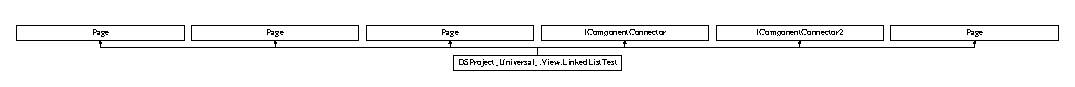
\includegraphics[height=0.720721cm]{class_d_s_project___universal___1_1_view_1_1_linked_list_test}
\end{center}
\end{figure}
\subsection*{Public Member Functions}
\begin{DoxyCompactItemize}
\item 
void \textbf{ Initialize\+Component} ()
\begin{DoxyCompactList}\small\item\em \doxyref{Initialize\+Component()}{p.}{class_d_s_project___universal___1_1_view_1_1_linked_list_test_adc7124594f63d3482048060f8ccc9d17} \end{DoxyCompactList}\item 
void \textbf{ Connect} (int connection\+Id, object target)
\begin{DoxyCompactList}\small\item\em \doxyref{Connect()}{p.}{class_d_s_project___universal___1_1_view_1_1_linked_list_test_a76d6534a4d1f0df72075b02e771fa486} \end{DoxyCompactList}\item 
\mbox{\label{class_d_s_project___universal___1_1_view_1_1_linked_list_test_acf190c4c65a8a3975cc5c70dddaede28}} 
global\+::\+Windows.\+U\+I.\+Xaml.\+Markup.\+I\+Component\+Connector {\bfseries Get\+Binding\+Connector} (int connection\+Id, object target)
\item 
void \textbf{ Initialize\+Component} ()
\begin{DoxyCompactList}\small\item\em \doxyref{Initialize\+Component()}{p.}{class_d_s_project___universal___1_1_view_1_1_linked_list_test_adc7124594f63d3482048060f8ccc9d17} \end{DoxyCompactList}\end{DoxyCompactItemize}
\subsection*{Protected Member Functions}
\begin{DoxyCompactItemize}
\item 
\mbox{\label{class_d_s_project___universal___1_1_view_1_1_linked_list_test_ac5057a27e1ac8c0cbfb176e0569f2f58}} 
async override void {\bfseries On\+Navigated\+To} (Navigation\+Event\+Args e)
\end{DoxyCompactItemize}


\subsection{Detailed Description}
An empty page that can be used on its own or navigated to within a Frame. 



\subsection{Member Function Documentation}
\mbox{\label{class_d_s_project___universal___1_1_view_1_1_linked_list_test_a76d6534a4d1f0df72075b02e771fa486}} 
\index{D\+S\+Project\+\_\+\+Universal\+\_\+\+::\+View\+::\+Linked\+List\+Test@{D\+S\+Project\+\_\+\+Universal\+\_\+\+::\+View\+::\+Linked\+List\+Test}!Connect@{Connect}}
\index{Connect@{Connect}!D\+S\+Project\+\_\+\+Universal\+\_\+\+::\+View\+::\+Linked\+List\+Test@{D\+S\+Project\+\_\+\+Universal\+\_\+\+::\+View\+::\+Linked\+List\+Test}}
\subsubsection{Connect()}
{\footnotesize\ttfamily void D\+S\+Project\+\_\+\+Universal\+\_\+.\+View.\+Linked\+List\+Test.\+Connect (\begin{DoxyParamCaption}\item[{int}]{connection\+Id,  }\item[{object}]{target }\end{DoxyParamCaption})}



\doxyref{Connect()}{p.}{class_d_s_project___universal___1_1_view_1_1_linked_list_test_a76d6534a4d1f0df72075b02e771fa486} 

\mbox{\label{class_d_s_project___universal___1_1_view_1_1_linked_list_test_adc7124594f63d3482048060f8ccc9d17}} 
\index{D\+S\+Project\+\_\+\+Universal\+\_\+\+::\+View\+::\+Linked\+List\+Test@{D\+S\+Project\+\_\+\+Universal\+\_\+\+::\+View\+::\+Linked\+List\+Test}!Initialize\+Component@{Initialize\+Component}}
\index{Initialize\+Component@{Initialize\+Component}!D\+S\+Project\+\_\+\+Universal\+\_\+\+::\+View\+::\+Linked\+List\+Test@{D\+S\+Project\+\_\+\+Universal\+\_\+\+::\+View\+::\+Linked\+List\+Test}}
\subsubsection{Initialize\+Component()\hspace{0.1cm}{\footnotesize\ttfamily [1/2]}}
{\footnotesize\ttfamily void D\+S\+Project\+\_\+\+Universal\+\_\+.\+View.\+Linked\+List\+Test.\+Initialize\+Component (\begin{DoxyParamCaption}{ }\end{DoxyParamCaption})}



\doxyref{Initialize\+Component()}{p.}{class_d_s_project___universal___1_1_view_1_1_linked_list_test_adc7124594f63d3482048060f8ccc9d17} 

\mbox{\label{class_d_s_project___universal___1_1_view_1_1_linked_list_test_adc7124594f63d3482048060f8ccc9d17}} 
\index{D\+S\+Project\+\_\+\+Universal\+\_\+\+::\+View\+::\+Linked\+List\+Test@{D\+S\+Project\+\_\+\+Universal\+\_\+\+::\+View\+::\+Linked\+List\+Test}!Initialize\+Component@{Initialize\+Component}}
\index{Initialize\+Component@{Initialize\+Component}!D\+S\+Project\+\_\+\+Universal\+\_\+\+::\+View\+::\+Linked\+List\+Test@{D\+S\+Project\+\_\+\+Universal\+\_\+\+::\+View\+::\+Linked\+List\+Test}}
\subsubsection{Initialize\+Component()\hspace{0.1cm}{\footnotesize\ttfamily [2/2]}}
{\footnotesize\ttfamily void D\+S\+Project\+\_\+\+Universal\+\_\+.\+View.\+Linked\+List\+Test.\+Initialize\+Component (\begin{DoxyParamCaption}{ }\end{DoxyParamCaption})}



\doxyref{Initialize\+Component()}{p.}{class_d_s_project___universal___1_1_view_1_1_linked_list_test_adc7124594f63d3482048060f8ccc9d17} 



The documentation for this class was generated from the following files\+:\begin{DoxyCompactItemize}
\item 
C\+:/\+Users/\+Sami/source/repos/\+D\+S\+Project(\+Universal)/\+D\+S\+Project(\+Universal)/obj/x64/\+Debug/\+View/.\+g.\+i.\+cs\item 
C\+:/\+Users/\+Sami/source/repos/\+D\+S\+Project(\+Universal)/\+D\+S\+Project(\+Universal)/obj/x64/\+Debug/\+View/Linked\+List\+Test.\+g.\+i.\+cs\item 
C\+:/\+Users/\+Sami/source/repos/\+D\+S\+Project(\+Universal)/\+D\+S\+Project(\+Universal)/obj/x64/\+Debug/\+View/Linked\+List\+Test.\+g.\+cs\item 
C\+:/\+Users/\+Sami/source/repos/\+D\+S\+Project(\+Universal)/\+D\+S\+Project(\+Universal)/\+View/Linked\+List\+Test.\+xaml.\+cs\end{DoxyCompactItemize}

\section{D\+S\+Project\+\_\+\+Universal\+\_\+.\+Main\+Page Class Reference}
\label{class_d_s_project___universal___1_1_main_page}\index{D\+S\+Project\+\_\+\+Universal\+\_\+.\+Main\+Page@{D\+S\+Project\+\_\+\+Universal\+\_\+.\+Main\+Page}}


An empty page that can be used on its own or navigated to within a Frame.  


Inheritance diagram for D\+S\+Project\+\_\+\+Universal\+\_\+.\+Main\+Page\+:\begin{figure}[H]
\begin{center}
\leavevmode
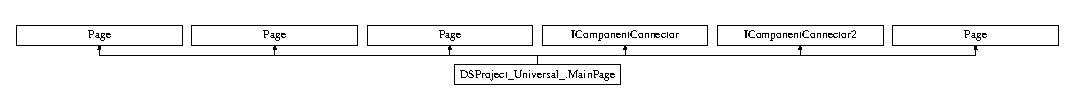
\includegraphics[height=0.910569cm]{class_d_s_project___universal___1_1_main_page}
\end{center}
\end{figure}
\subsection*{Public Member Functions}
\begin{DoxyCompactItemize}
\item 
void \textbf{ Connect} (int connection\+Id, object target)
\begin{DoxyCompactList}\small\item\em \doxyref{Connect()}{p.}{class_d_s_project___universal___1_1_main_page_af5a22f0a255fa0442561d2deeaa1559d} \end{DoxyCompactList}\item 
\mbox{\label{class_d_s_project___universal___1_1_main_page_a67a47186e429b51fff89d3fad5769762}} 
global\+::\+Windows.\+U\+I.\+Xaml.\+Markup.\+I\+Component\+Connector {\bfseries Get\+Binding\+Connector} (int connection\+Id, object target)
\item 
void \textbf{ Initialize\+Component} ()
\begin{DoxyCompactList}\small\item\em \doxyref{Initialize\+Component()}{p.}{class_d_s_project___universal___1_1_main_page_a31f00c607367c0a3747d15995e628b0d} \end{DoxyCompactList}\item 
void \textbf{ Initialize\+Component} ()
\begin{DoxyCompactList}\small\item\em \doxyref{Initialize\+Component()}{p.}{class_d_s_project___universal___1_1_main_page_a31f00c607367c0a3747d15995e628b0d} \end{DoxyCompactList}\end{DoxyCompactItemize}


\subsection{Detailed Description}
An empty page that can be used on its own or navigated to within a Frame. 



\subsection{Member Function Documentation}
\mbox{\label{class_d_s_project___universal___1_1_main_page_af5a22f0a255fa0442561d2deeaa1559d}} 
\index{D\+S\+Project\+\_\+\+Universal\+\_\+\+::\+Main\+Page@{D\+S\+Project\+\_\+\+Universal\+\_\+\+::\+Main\+Page}!Connect@{Connect}}
\index{Connect@{Connect}!D\+S\+Project\+\_\+\+Universal\+\_\+\+::\+Main\+Page@{D\+S\+Project\+\_\+\+Universal\+\_\+\+::\+Main\+Page}}
\subsubsection{Connect()}
{\footnotesize\ttfamily void D\+S\+Project\+\_\+\+Universal\+\_\+.\+Main\+Page.\+Connect (\begin{DoxyParamCaption}\item[{int}]{connection\+Id,  }\item[{object}]{target }\end{DoxyParamCaption})}



\doxyref{Connect()}{p.}{class_d_s_project___universal___1_1_main_page_af5a22f0a255fa0442561d2deeaa1559d} 

\mbox{\label{class_d_s_project___universal___1_1_main_page_a31f00c607367c0a3747d15995e628b0d}} 
\index{D\+S\+Project\+\_\+\+Universal\+\_\+\+::\+Main\+Page@{D\+S\+Project\+\_\+\+Universal\+\_\+\+::\+Main\+Page}!Initialize\+Component@{Initialize\+Component}}
\index{Initialize\+Component@{Initialize\+Component}!D\+S\+Project\+\_\+\+Universal\+\_\+\+::\+Main\+Page@{D\+S\+Project\+\_\+\+Universal\+\_\+\+::\+Main\+Page}}
\subsubsection{Initialize\+Component()\hspace{0.1cm}{\footnotesize\ttfamily [1/2]}}
{\footnotesize\ttfamily void D\+S\+Project\+\_\+\+Universal\+\_\+.\+Main\+Page.\+Initialize\+Component (\begin{DoxyParamCaption}{ }\end{DoxyParamCaption})}



\doxyref{Initialize\+Component()}{p.}{class_d_s_project___universal___1_1_main_page_a31f00c607367c0a3747d15995e628b0d} 

\mbox{\label{class_d_s_project___universal___1_1_main_page_a31f00c607367c0a3747d15995e628b0d}} 
\index{D\+S\+Project\+\_\+\+Universal\+\_\+\+::\+Main\+Page@{D\+S\+Project\+\_\+\+Universal\+\_\+\+::\+Main\+Page}!Initialize\+Component@{Initialize\+Component}}
\index{Initialize\+Component@{Initialize\+Component}!D\+S\+Project\+\_\+\+Universal\+\_\+\+::\+Main\+Page@{D\+S\+Project\+\_\+\+Universal\+\_\+\+::\+Main\+Page}}
\subsubsection{Initialize\+Component()\hspace{0.1cm}{\footnotesize\ttfamily [2/2]}}
{\footnotesize\ttfamily void D\+S\+Project\+\_\+\+Universal\+\_\+.\+Main\+Page.\+Initialize\+Component (\begin{DoxyParamCaption}{ }\end{DoxyParamCaption})}



\doxyref{Initialize\+Component()}{p.}{class_d_s_project___universal___1_1_main_page_a31f00c607367c0a3747d15995e628b0d} 



The documentation for this class was generated from the following files\+:\begin{DoxyCompactItemize}
\item 
C\+:/\+Users/\+Sami/source/repos/\+D\+S\+Project(\+Universal)/\+D\+S\+Project(\+Universal)/Main\+Page.\+xaml.\+cs\item 
C\+:/\+Users/\+Sami/source/repos/\+D\+S\+Project(\+Universal)/\+D\+S\+Project(\+Universal)/obj/x64/\+Debug/Main\+Page.\+g.\+i.\+cs\item 
C\+:/\+Users/\+Sami/source/repos/\+D\+S\+Project(\+Universal)/\+D\+S\+Project(\+Universal)/obj/x64/\+Debug/Main\+Page.\+g.\+cs\end{DoxyCompactItemize}

\section{D\+S\+Project\+Universal.\+Util.\+Node$<$ T $>$ Class Template Reference}
\label{class_d_s_project_universal_1_1_util_1_1_node}\index{D\+S\+Project\+Universal.\+Util.\+Node$<$ T $>$@{D\+S\+Project\+Universal.\+Util.\+Node$<$ T $>$}}


Class of objects representing nodes of a linked list 


\subsection*{Public Member Functions}
\begin{DoxyCompactItemize}
\item 
\mbox{\label{class_d_s_project_universal_1_1_util_1_1_node_a642b6a15d69d74741ebfbed85c6f40bd}} 
\textbf{ Node} ()
\begin{DoxyCompactList}\small\item\em Sets pointers to next and previous nodes in list to false\end{DoxyCompactList}\item 
\mbox{\label{class_d_s_project_universal_1_1_util_1_1_node_a5b3fc6028f3199fe82e1876507dd5c2c}} 
\textbf{ Node} (T data)
\begin{DoxyCompactList}\small\item\em Sets data of node to the given data\end{DoxyCompactList}\item 
\mbox{\label{class_d_s_project_universal_1_1_util_1_1_node_af84b42c7b9dc39eaf0b2f1dc5a1b1a8d}} 
\textbf{ Node} (T data, \textbf{ Node}$<$ T $>$ previous)
\begin{DoxyCompactList}\small\item\em Sets data and pointer to previous node of list to given values\end{DoxyCompactList}\item 
\mbox{\label{class_d_s_project_universal_1_1_util_1_1_node_aa19f0eb3f55f3016aac255cfc0d717e5}} 
\textbf{ Node} (T data, \textbf{ Node}$<$ T $>$ previous, \textbf{ Node}$<$ T $>$ next)
\begin{DoxyCompactList}\small\item\em Sets data and pointers to previous and next nodes on list to given values\end{DoxyCompactList}\item 
\textbf{ Node}$<$ T $>$ \textbf{ Set\+Next} (\textbf{ Node}$<$ T $>$ next)
\begin{DoxyCompactList}\small\item\em Sets pointer to next node on list to given value\end{DoxyCompactList}\item 
\textbf{ Node}$<$ T $>$ \textbf{ Set\+Previous} (\textbf{ Node}$<$ T $>$ previous)
\begin{DoxyCompactList}\small\item\em Sets pointer to previious node on list to given value\end{DoxyCompactList}\item 
\textbf{ Node}$<$ T $>$ \textbf{ Set\+Data} (T data)
\begin{DoxyCompactList}\small\item\em Sets data of node to given value\end{DoxyCompactList}\end{DoxyCompactItemize}
\subsection*{Properties}
\begin{DoxyCompactItemize}
\item 
\mbox{\label{class_d_s_project_universal_1_1_util_1_1_node_a0fa5e552e505eafe3b17b8624929560c}} 
\textbf{ Node}$<$ T $>$ \textbf{ Next}\hspace{0.3cm}{\ttfamily  [get]}
\begin{DoxyCompactList}\small\item\em Pointer to next node in list\end{DoxyCompactList}\item 
\mbox{\label{class_d_s_project_universal_1_1_util_1_1_node_aa77750e081a6e6f6ec16f3628cd3610f}} 
\textbf{ Node}$<$ T $>$ \textbf{ Previous}\hspace{0.3cm}{\ttfamily  [get]}
\begin{DoxyCompactList}\small\item\em Pointer to previous node in list\end{DoxyCompactList}\item 
\mbox{\label{class_d_s_project_universal_1_1_util_1_1_node_ab0dbcdfe94ab49f8e5e4b8a4c0be424e}} 
T \textbf{ Data}\hspace{0.3cm}{\ttfamily  [get]}
\begin{DoxyCompactList}\small\item\em Data object of the node to store any kind of data\end{DoxyCompactList}\end{DoxyCompactItemize}


\subsection{Detailed Description}
Class of objects representing nodes of a linked list

\subsection{Member Function Documentation}
\mbox{\label{class_d_s_project_universal_1_1_util_1_1_node_a8b9228c07f419757b125647f43bf1172}} 
\index{D\+S\+Project\+Universal\+::\+Util\+::\+Node@{D\+S\+Project\+Universal\+::\+Util\+::\+Node}!Set\+Data@{Set\+Data}}
\index{Set\+Data@{Set\+Data}!D\+S\+Project\+Universal\+::\+Util\+::\+Node@{D\+S\+Project\+Universal\+::\+Util\+::\+Node}}
\subsubsection{Set\+Data()}
{\footnotesize\ttfamily \textbf{ Node}$<$T$>$ \textbf{ D\+S\+Project\+Universal.\+Util.\+Node}$<$ T $>$.Set\+Data (\begin{DoxyParamCaption}\item[{T}]{data }\end{DoxyParamCaption})}



Sets data of node to given value


\begin{DoxyParams}{Parameters}
{\em data} & The data we are setting node\textquotesingle{}s data to\\
\hline
\end{DoxyParams}
\begin{DoxyReturn}{Returns}
Reference to the very node
\end{DoxyReturn}
\mbox{\label{class_d_s_project_universal_1_1_util_1_1_node_ad7f94be406fda024110172063732f15f}} 
\index{D\+S\+Project\+Universal\+::\+Util\+::\+Node@{D\+S\+Project\+Universal\+::\+Util\+::\+Node}!Set\+Next@{Set\+Next}}
\index{Set\+Next@{Set\+Next}!D\+S\+Project\+Universal\+::\+Util\+::\+Node@{D\+S\+Project\+Universal\+::\+Util\+::\+Node}}
\subsubsection{Set\+Next()}
{\footnotesize\ttfamily \textbf{ Node}$<$T$>$ \textbf{ D\+S\+Project\+Universal.\+Util.\+Node}$<$ T $>$.Set\+Next (\begin{DoxyParamCaption}\item[{\textbf{ Node}$<$ T $>$}]{next }\end{DoxyParamCaption})}



Sets pointer to next node on list to given value


\begin{DoxyParams}{Parameters}
{\em next} & Reference to the node set to be pointer to next node on list\\
\hline
\end{DoxyParams}
\begin{DoxyReturn}{Returns}
Reference to the very node
\end{DoxyReturn}
\mbox{\label{class_d_s_project_universal_1_1_util_1_1_node_acb8111bb0b6db39c5e872498b9c42059}} 
\index{D\+S\+Project\+Universal\+::\+Util\+::\+Node@{D\+S\+Project\+Universal\+::\+Util\+::\+Node}!Set\+Previous@{Set\+Previous}}
\index{Set\+Previous@{Set\+Previous}!D\+S\+Project\+Universal\+::\+Util\+::\+Node@{D\+S\+Project\+Universal\+::\+Util\+::\+Node}}
\subsubsection{Set\+Previous()}
{\footnotesize\ttfamily \textbf{ Node}$<$T$>$ \textbf{ D\+S\+Project\+Universal.\+Util.\+Node}$<$ T $>$.Set\+Previous (\begin{DoxyParamCaption}\item[{\textbf{ Node}$<$ T $>$}]{previous }\end{DoxyParamCaption})}



Sets pointer to previious node on list to given value


\begin{DoxyParams}{Parameters}
{\em previous} & Reference to the node set to be pointer to previous node on list\\
\hline
\end{DoxyParams}
\begin{DoxyReturn}{Returns}
Reference to the very node
\end{DoxyReturn}


The documentation for this class was generated from the following file\+:\begin{DoxyCompactItemize}
\item 
C\+:/\+Users/\+Sami/source/repos/\+D\+S\+Project(\+Universal)/\+D\+S\+Project(\+Universal)/\+Util/Linked\+List.\+cs\end{DoxyCompactItemize}

\section{D\+S\+Project\+\_\+\+Universal\+\_\+.\+View.\+Root\+Page Class Reference}
\label{class_d_s_project___universal___1_1_view_1_1_root_page}\index{D\+S\+Project\+\_\+\+Universal\+\_\+.\+View.\+Root\+Page@{D\+S\+Project\+\_\+\+Universal\+\_\+.\+View.\+Root\+Page}}


An empty page that can be used on its own or navigated to within a Frame.  


Inheritance diagram for D\+S\+Project\+\_\+\+Universal\+\_\+.\+View.\+Root\+Page\+:\begin{figure}[H]
\begin{center}
\leavevmode
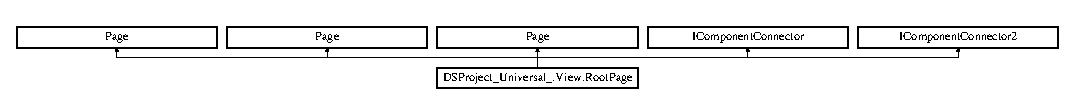
\includegraphics[height=0.957265cm]{class_d_s_project___universal___1_1_view_1_1_root_page}
\end{center}
\end{figure}
\subsection*{Public Member Functions}
\begin{DoxyCompactItemize}
\item 
void \textbf{ Connect} (int connection\+Id, object target)
\begin{DoxyCompactList}\small\item\em \doxyref{Connect()}{p.}{class_d_s_project___universal___1_1_view_1_1_root_page_a79abe803b00bf714ff18ca617b438f70} \end{DoxyCompactList}\item 
\mbox{\label{class_d_s_project___universal___1_1_view_1_1_root_page_aff63baf9f003ef75133d7b90269d84bd}} 
global\+::\+Windows.\+U\+I.\+Xaml.\+Markup.\+I\+Component\+Connector {\bfseries Get\+Binding\+Connector} (int connection\+Id, object target)
\item 
void \textbf{ Initialize\+Component} ()
\begin{DoxyCompactList}\small\item\em \doxyref{Initialize\+Component()}{p.}{class_d_s_project___universal___1_1_view_1_1_root_page_a9c15764baa2dbda73f84a3499f060fc5} \end{DoxyCompactList}\end{DoxyCompactItemize}
\subsection*{Protected Member Functions}
\begin{DoxyCompactItemize}
\item 
\mbox{\label{class_d_s_project___universal___1_1_view_1_1_root_page_a5760fdfd609b6dd5f3ac146d86a859cf}} 
override void {\bfseries On\+Navigated\+To} (Navigation\+Event\+Args e)
\end{DoxyCompactItemize}


\subsection{Detailed Description}
An empty page that can be used on its own or navigated to within a Frame. 



\subsection{Member Function Documentation}
\mbox{\label{class_d_s_project___universal___1_1_view_1_1_root_page_a79abe803b00bf714ff18ca617b438f70}} 
\index{D\+S\+Project\+\_\+\+Universal\+\_\+\+::\+View\+::\+Root\+Page@{D\+S\+Project\+\_\+\+Universal\+\_\+\+::\+View\+::\+Root\+Page}!Connect@{Connect}}
\index{Connect@{Connect}!D\+S\+Project\+\_\+\+Universal\+\_\+\+::\+View\+::\+Root\+Page@{D\+S\+Project\+\_\+\+Universal\+\_\+\+::\+View\+::\+Root\+Page}}
\subsubsection{Connect()}
{\footnotesize\ttfamily void D\+S\+Project\+\_\+\+Universal\+\_\+.\+View.\+Root\+Page.\+Connect (\begin{DoxyParamCaption}\item[{int}]{connection\+Id,  }\item[{object}]{target }\end{DoxyParamCaption})}



\doxyref{Connect()}{p.}{class_d_s_project___universal___1_1_view_1_1_root_page_a79abe803b00bf714ff18ca617b438f70} 

\mbox{\label{class_d_s_project___universal___1_1_view_1_1_root_page_a9c15764baa2dbda73f84a3499f060fc5}} 
\index{D\+S\+Project\+\_\+\+Universal\+\_\+\+::\+View\+::\+Root\+Page@{D\+S\+Project\+\_\+\+Universal\+\_\+\+::\+View\+::\+Root\+Page}!Initialize\+Component@{Initialize\+Component}}
\index{Initialize\+Component@{Initialize\+Component}!D\+S\+Project\+\_\+\+Universal\+\_\+\+::\+View\+::\+Root\+Page@{D\+S\+Project\+\_\+\+Universal\+\_\+\+::\+View\+::\+Root\+Page}}
\subsubsection{Initialize\+Component()}
{\footnotesize\ttfamily void D\+S\+Project\+\_\+\+Universal\+\_\+.\+View.\+Root\+Page.\+Initialize\+Component (\begin{DoxyParamCaption}{ }\end{DoxyParamCaption})}



\doxyref{Initialize\+Component()}{p.}{class_d_s_project___universal___1_1_view_1_1_root_page_a9c15764baa2dbda73f84a3499f060fc5} 



The documentation for this class was generated from the following files\+:\begin{DoxyCompactItemize}
\item 
C\+:/\+Users/\+Sami/source/repos/\+D\+S\+Project(\+Universal)/\+D\+S\+Project(\+Universal)/obj/x64/\+Debug/\+View/Root\+Page.\+g.\+cs\item 
C\+:/\+Users/\+Sami/source/repos/\+D\+S\+Project(\+Universal)/\+D\+S\+Project(\+Universal)/obj/x64/\+Debug/\+View/Root\+Page.\+g.\+i.\+cs\item 
C\+:/\+Users/\+Sami/source/repos/\+D\+S\+Project(\+Universal)/\+D\+S\+Project(\+Universal)/\+View/Root\+Page.\+xaml.\+cs\end{DoxyCompactItemize}

\section{D\+S\+Project\+Universal.\+Model.\+Service Class Reference}
\label{class_d_s_project_universal_1_1_model_1_1_service}\index{D\+S\+Project\+Universal.\+Model.\+Service@{D\+S\+Project\+Universal.\+Model.\+Service}}
Inheritance diagram for D\+S\+Project\+Universal.\+Model.\+Service\+:\begin{figure}[H]
\begin{center}
\leavevmode
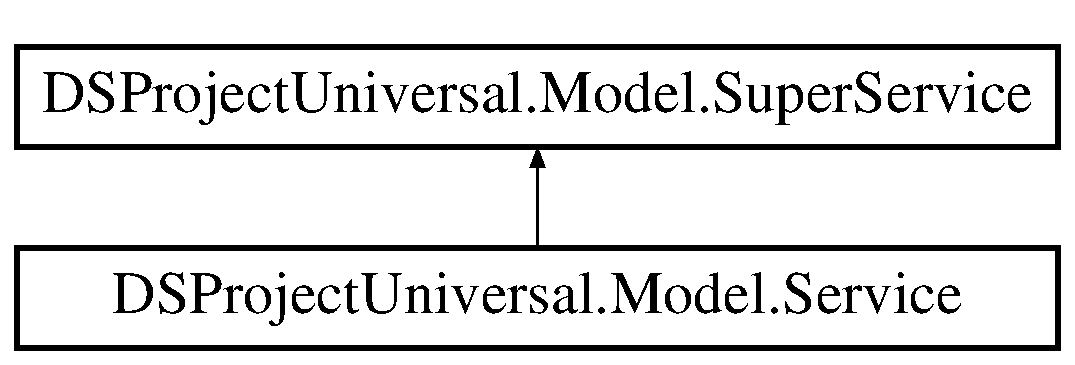
\includegraphics[height=2.000000cm]{class_d_s_project_universal_1_1_model_1_1_service}
\end{center}
\end{figure}
\subsection*{Public Member Functions}
\begin{DoxyCompactItemize}
\item 
\mbox{\label{class_d_s_project_universal_1_1_model_1_1_service_aaa3c16f3a5caa57bd625ddb0bfe09d90}} 
{\bfseries Service} (string name, string cus\+Desc, string tech\+Desc, string car\+Model, int expence, int id)
\item 
\mbox{\label{class_d_s_project_universal_1_1_model_1_1_service_ae17df2a3b411424c78079d06faf06387}} 
\textbf{ Service} {\bfseries Add\+Sub\+Service} (\textbf{ Sub\+Service} sub\+Service)
\item 
override bool \textbf{ Has\+Dependency} (int id)
\begin{DoxyCompactList}\small\item\em Checks service or subservice if it has a subservice in its subservices recursivly\end{DoxyCompactList}\item 
\mbox{\label{class_d_s_project_universal_1_1_model_1_1_service_a2e93eb733accd8fd129e4c5244b3fb5b}} 
\textbf{ Service} {\bfseries Remove\+Subservice} (\textbf{ Sub\+Service} sub\+Service)
\item 
\mbox{\label{class_d_s_project_universal_1_1_model_1_1_service_a07df67de6217c07575318135a1ef166f}} 
void {\bfseries Delete} ()
\end{DoxyCompactItemize}
\subsection*{Properties}
\begin{DoxyCompactItemize}
\item 
\mbox{\label{class_d_s_project_universal_1_1_model_1_1_service_a3cb87904dbdacc494ca1becece518818}} 
string {\bfseries Customer\+Description}\hspace{0.3cm}{\ttfamily  [get]}
\item 
\mbox{\label{class_d_s_project_universal_1_1_model_1_1_service_a053e3a28ca06aba5496c9197c6212f5d}} 
string {\bfseries Technical\+Description}\hspace{0.3cm}{\ttfamily  [get]}
\item 
\mbox{\label{class_d_s_project_universal_1_1_model_1_1_service_a6611b789f5dfd5ee2d26692ad5602984}} 
string {\bfseries Car\+Model}\hspace{0.3cm}{\ttfamily  [get]}
\item 
\mbox{\label{class_d_s_project_universal_1_1_model_1_1_service_ad0730be4535e107e76bea27f7797e30f}} 
int {\bfseries Expence}\hspace{0.3cm}{\ttfamily  [get]}
\item 
\mbox{\label{class_d_s_project_universal_1_1_model_1_1_service_aa4f89a5b851cbeaf24e5a51a78787578}} 
\textbf{ Linked\+List}$<$ \textbf{ Sub\+Service} $>$ {\bfseries Sub\+Services}\hspace{0.3cm}{\ttfamily  [get]}
\end{DoxyCompactItemize}


\subsection{Member Function Documentation}
\mbox{\label{class_d_s_project_universal_1_1_model_1_1_service_af4c682317779dba6e27be35d50f236c9}} 
\index{D\+S\+Project\+Universal\+::\+Model\+::\+Service@{D\+S\+Project\+Universal\+::\+Model\+::\+Service}!Has\+Dependency@{Has\+Dependency}}
\index{Has\+Dependency@{Has\+Dependency}!D\+S\+Project\+Universal\+::\+Model\+::\+Service@{D\+S\+Project\+Universal\+::\+Model\+::\+Service}}
\subsubsection{Has\+Dependency()}
{\footnotesize\ttfamily override bool D\+S\+Project\+Universal.\+Model.\+Service.\+Has\+Dependency (\begin{DoxyParamCaption}\item[{int}]{id }\end{DoxyParamCaption})\hspace{0.3cm}{\ttfamily [virtual]}}



Checks service or subservice if it has a subservice in its subservices recursivly


\begin{DoxyParams}{Parameters}
{\em id} & ID of the subservice we are looking for\\
\hline
\end{DoxyParams}
\begin{DoxyReturn}{Returns}
Returns true if it has the subservice and return false otherwise
\end{DoxyReturn}


Implements \textbf{ D\+S\+Project\+Universal.\+Model.\+Super\+Service} \doxyref{}{p.}{class_d_s_project_universal_1_1_model_1_1_super_service_a617b1309bed57798f76a71eac6ec6e11}.



The documentation for this class was generated from the following file\+:\begin{DoxyCompactItemize}
\item 
C\+:/\+Users/\+Sami/source/repos/\+D\+S\+Project(\+Universal)/\+D\+S\+Project(\+Universal)/\+Model/Service.\+cs\end{DoxyCompactItemize}

\section{D\+S\+Project\+Universal.\+Model.\+Service\+Pool Class Reference}
\label{class_d_s_project_universal_1_1_model_1_1_service_pool}\index{D\+S\+Project\+Universal.\+Model.\+Service\+Pool@{D\+S\+Project\+Universal.\+Model.\+Service\+Pool}}


A place to store all active services 


\subsection*{Public Member Functions}
\begin{DoxyCompactItemize}
\item 
\mbox{\label{class_d_s_project_universal_1_1_model_1_1_service_pool_af88bf88a9e6c1687be48b2e00cce28be}} 
\textbf{ Service\+Pool} ()
\begin{DoxyCompactList}\small\item\em Creating list object\end{DoxyCompactList}\item 
\mbox{\label{class_d_s_project_universal_1_1_model_1_1_service_pool_aed73511deb8179e675e445ccb05d866a}} 
\textbf{ Service\+Pool} \textbf{ Add\+Service} (\textbf{ Service} service)
\begin{DoxyCompactList}\small\item\em Adds a service in active services list\end{DoxyCompactList}\item 
\mbox{\label{class_d_s_project_universal_1_1_model_1_1_service_pool_a4c48b001f40bffd91887bf2bcc1dd2d4}} 
\textbf{ Service\+Pool} \textbf{ Remove\+Service} (\textbf{ Service} service)
\begin{DoxyCompactList}\small\item\em Removes a service from active services\end{DoxyCompactList}\item 
\textbf{ Service} \textbf{ Get\+Service} (int id)
\begin{DoxyCompactList}\small\item\em Finds an active service by ID\end{DoxyCompactList}\end{DoxyCompactItemize}
\subsection*{Public Attributes}
\begin{DoxyCompactItemize}
\item 
\mbox{\label{class_d_s_project_universal_1_1_model_1_1_service_pool_a796c40b943c1b5872d10d87dfca4e869}} 
int \textbf{ Length} =$>$ List.\+Length
\begin{DoxyCompactList}\small\item\em Return number of active services\end{DoxyCompactList}\end{DoxyCompactItemize}


\subsection{Detailed Description}
A place to store all active services

\subsection{Member Function Documentation}
\mbox{\label{class_d_s_project_universal_1_1_model_1_1_service_pool_ae63e3905a9b4396923ac8fa6792dd83d}} 
\index{D\+S\+Project\+Universal\+::\+Model\+::\+Service\+Pool@{D\+S\+Project\+Universal\+::\+Model\+::\+Service\+Pool}!Get\+Service@{Get\+Service}}
\index{Get\+Service@{Get\+Service}!D\+S\+Project\+Universal\+::\+Model\+::\+Service\+Pool@{D\+S\+Project\+Universal\+::\+Model\+::\+Service\+Pool}}
\subsubsection{Get\+Service()}
{\footnotesize\ttfamily \textbf{ Service} D\+S\+Project\+Universal.\+Model.\+Service\+Pool.\+Get\+Service (\begin{DoxyParamCaption}\item[{int}]{id }\end{DoxyParamCaption})}



Finds an active service by ID


\begin{DoxyParams}{Parameters}
{\em id} & ID of the service we are looking for\\
\hline
\end{DoxyParams}


Finds with O(n)

\begin{DoxyReturn}{Returns}
The service with given ID
\end{DoxyReturn}


The documentation for this class was generated from the following file\+:\begin{DoxyCompactItemize}
\item 
C\+:/\+Users/\+Sami/source/repos/\+D\+S\+Project(\+Universal)/\+D\+S\+Project(\+Universal)/\+Model/Pool.\+cs\end{DoxyCompactItemize}

\section{D\+S\+Project\+Universal.\+Model.\+Sub\+Service Class Reference}
\label{class_d_s_project_universal_1_1_model_1_1_sub_service}\index{D\+S\+Project\+Universal.\+Model.\+Sub\+Service@{D\+S\+Project\+Universal.\+Model.\+Sub\+Service}}
Inheritance diagram for D\+S\+Project\+Universal.\+Model.\+Sub\+Service\+:\begin{figure}[H]
\begin{center}
\leavevmode
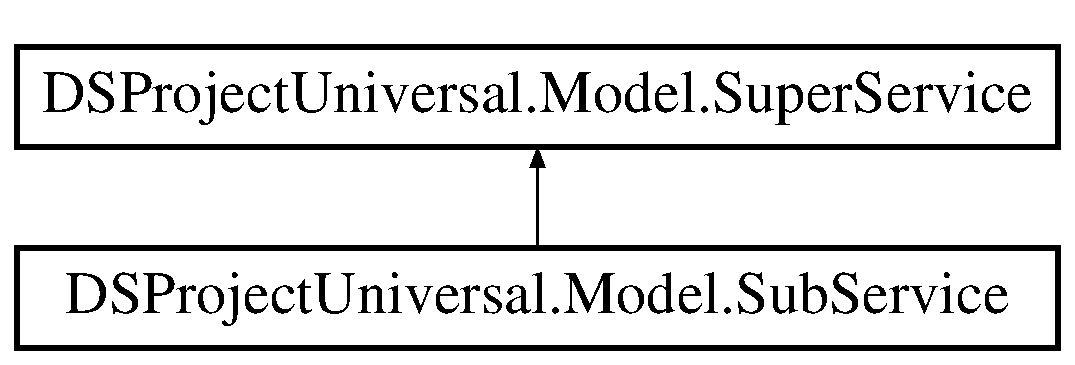
\includegraphics[height=2.000000cm]{class_d_s_project_universal_1_1_model_1_1_sub_service}
\end{center}
\end{figure}
\subsection*{Public Member Functions}
\begin{DoxyCompactItemize}
\item 
\mbox{\label{class_d_s_project_universal_1_1_model_1_1_sub_service_a77885b70e3c29cf05bf28f1eb9ca8e4c}} 
{\bfseries Sub\+Service} (string name, int id)
\item 
override bool \textbf{ Has\+Dependency} (int id)
\begin{DoxyCompactList}\small\item\em Checks service or subservice if it has a subservice in its subservices recursivly\end{DoxyCompactList}\item 
\mbox{\label{class_d_s_project_universal_1_1_model_1_1_sub_service_a02914c7288dcd49bac694567a84fea35}} 
\textbf{ Sub\+Service} {\bfseries Add\+Parrent} (\textbf{ Super\+Service} parrent)
\item 
\mbox{\label{class_d_s_project_universal_1_1_model_1_1_sub_service_a24d5f8266abb16dc7a62c0bb676d39a6}} 
\textbf{ Sub\+Service} {\bfseries Romove\+Parent} (\textbf{ Super\+Service} parent)
\end{DoxyCompactItemize}
\subsection*{Additional Inherited Members}


\subsection{Member Function Documentation}
\mbox{\label{class_d_s_project_universal_1_1_model_1_1_sub_service_adae90aa35f26ca0ce8ff4ed6439b890e}} 
\index{D\+S\+Project\+Universal\+::\+Model\+::\+Sub\+Service@{D\+S\+Project\+Universal\+::\+Model\+::\+Sub\+Service}!Has\+Dependency@{Has\+Dependency}}
\index{Has\+Dependency@{Has\+Dependency}!D\+S\+Project\+Universal\+::\+Model\+::\+Sub\+Service@{D\+S\+Project\+Universal\+::\+Model\+::\+Sub\+Service}}
\subsubsection{Has\+Dependency()}
{\footnotesize\ttfamily override bool D\+S\+Project\+Universal.\+Model.\+Sub\+Service.\+Has\+Dependency (\begin{DoxyParamCaption}\item[{int}]{id }\end{DoxyParamCaption})\hspace{0.3cm}{\ttfamily [virtual]}}



Checks service or subservice if it has a subservice in its subservices recursivly


\begin{DoxyParams}{Parameters}
{\em id} & ID of the subservice we are looking for\\
\hline
\end{DoxyParams}
\begin{DoxyReturn}{Returns}
Returns true if it has the subservice and return false otherwise
\end{DoxyReturn}


Implements \textbf{ D\+S\+Project\+Universal.\+Model.\+Super\+Service} \doxyref{}{p.}{class_d_s_project_universal_1_1_model_1_1_super_service_a617b1309bed57798f76a71eac6ec6e11}.



The documentation for this class was generated from the following file\+:\begin{DoxyCompactItemize}
\item 
C\+:/\+Users/\+Sami/source/repos/\+D\+S\+Project(\+Universal)/\+D\+S\+Project(\+Universal)/\+Model/Service.\+cs\end{DoxyCompactItemize}

\section{D\+S\+Project\+Universal.\+Model.\+Sub\+Service\+Pool Class Reference}
\label{class_d_s_project_universal_1_1_model_1_1_sub_service_pool}\index{D\+S\+Project\+Universal.\+Model.\+Sub\+Service\+Pool@{D\+S\+Project\+Universal.\+Model.\+Sub\+Service\+Pool}}


A place to store all active subservices 


\subsection*{Public Member Functions}
\begin{DoxyCompactItemize}
\item 
\mbox{\label{class_d_s_project_universal_1_1_model_1_1_sub_service_pool_aaf0770dba1193da180858c6a16f87750}} 
\textbf{ Sub\+Service\+Pool} ()
\begin{DoxyCompactList}\small\item\em Creates list object to store subservices\end{DoxyCompactList}\item 
\mbox{\label{class_d_s_project_universal_1_1_model_1_1_sub_service_pool_afe561c40615586058410baba5cbd7bf4}} 
\textbf{ Sub\+Service\+Pool} \textbf{ Add\+Sub\+Service} (\textbf{ Sub\+Service} sub\+Service)
\begin{DoxyCompactList}\small\item\em Add a sub service to active subservices list\end{DoxyCompactList}\item 
\mbox{\label{class_d_s_project_universal_1_1_model_1_1_sub_service_pool_a20888fbce0c4a9f79a576c6fb4963458}} 
\textbf{ Sub\+Service\+Pool} \textbf{ Remove\+Sub\+Service} (\textbf{ Sub\+Service} sub\+Service)
\begin{DoxyCompactList}\small\item\em Removes a subservice from active subservices list\end{DoxyCompactList}\item 
\textbf{ Sub\+Service} \textbf{ Get\+Sub\+Service} (int id)
\begin{DoxyCompactList}\small\item\em Finds a subservice by ID\end{DoxyCompactList}\end{DoxyCompactItemize}
\subsection*{Public Attributes}
\begin{DoxyCompactItemize}
\item 
\mbox{\label{class_d_s_project_universal_1_1_model_1_1_sub_service_pool_ae840475ba448fe2381a45dd7950ab108}} 
int \textbf{ Length} =$>$ List.\+Length
\begin{DoxyCompactList}\small\item\em Returns number of active subservices\end{DoxyCompactList}\end{DoxyCompactItemize}
\subsection*{Protected Attributes}
\begin{DoxyCompactItemize}
\item 
\mbox{\label{class_d_s_project_universal_1_1_model_1_1_sub_service_pool_ae35d08a93e4077d6c841152cf7052d55}} 
\textbf{ Linked\+List}$<$ \textbf{ Sub\+Service} $>$ \textbf{ List}
\begin{DoxyCompactList}\small\item\em Stores Super\+Services\end{DoxyCompactList}\end{DoxyCompactItemize}


\subsection{Detailed Description}
A place to store all active subservices

\subsection{Member Function Documentation}
\mbox{\label{class_d_s_project_universal_1_1_model_1_1_sub_service_pool_a3aefcae44f633d1c959fe6bd388c2ab8}} 
\index{D\+S\+Project\+Universal\+::\+Model\+::\+Sub\+Service\+Pool@{D\+S\+Project\+Universal\+::\+Model\+::\+Sub\+Service\+Pool}!Get\+Sub\+Service@{Get\+Sub\+Service}}
\index{Get\+Sub\+Service@{Get\+Sub\+Service}!D\+S\+Project\+Universal\+::\+Model\+::\+Sub\+Service\+Pool@{D\+S\+Project\+Universal\+::\+Model\+::\+Sub\+Service\+Pool}}
\subsubsection{Get\+Sub\+Service()}
{\footnotesize\ttfamily \textbf{ Sub\+Service} D\+S\+Project\+Universal.\+Model.\+Sub\+Service\+Pool.\+Get\+Sub\+Service (\begin{DoxyParamCaption}\item[{int}]{id }\end{DoxyParamCaption})}



Finds a subservice by ID


\begin{DoxyParams}{Parameters}
{\em id} & ID of subservice we are looking for\\
\hline
\end{DoxyParams}


Finds with O(n)

\begin{DoxyReturn}{Returns}
The subservice with the given ID
\end{DoxyReturn}


The documentation for this class was generated from the following file\+:\begin{DoxyCompactItemize}
\item 
C\+:/\+Users/\+Sami/source/repos/\+D\+S\+Project(\+Universal)/\+D\+S\+Project(\+Universal)/\+Model/Pool.\+cs\end{DoxyCompactItemize}

\section{D\+S\+Project\+Universal.\+Model.\+Super\+Service Class Reference}
\label{class_d_s_project_universal_1_1_model_1_1_super_service}\index{D\+S\+Project\+Universal.\+Model.\+Super\+Service@{D\+S\+Project\+Universal.\+Model.\+Super\+Service}}


An abstract represents services and subservices 


Inheritance diagram for D\+S\+Project\+Universal.\+Model.\+Super\+Service\+:\begin{figure}[H]
\begin{center}
\leavevmode
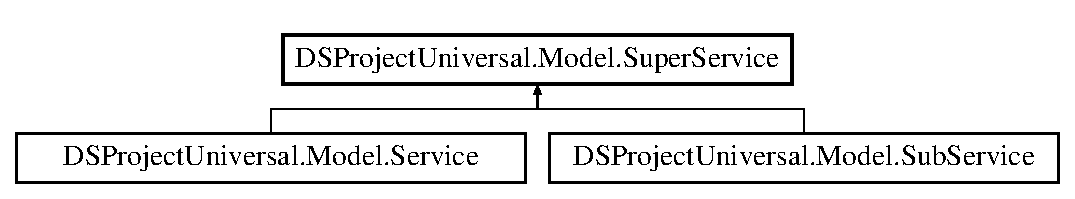
\includegraphics[height=2.000000cm]{class_d_s_project_universal_1_1_model_1_1_super_service}
\end{center}
\end{figure}
\subsection*{Public Member Functions}
\begin{DoxyCompactItemize}
\item 
\mbox{\label{class_d_s_project_universal_1_1_model_1_1_super_service_ae1aeb419a7909af6ef52794e942491ec}} 
\textbf{ Super\+Service} (string name, int id)
\begin{DoxyCompactList}\small\item\em Initializes ID and Name of current service or subservice with given ID and Name\end{DoxyCompactList}\item 
abstract bool \textbf{ Has\+Dependency} (int id)
\begin{DoxyCompactList}\small\item\em Checks service or subservice if it has a subservice in its subservices recursivly\end{DoxyCompactList}\end{DoxyCompactItemize}
\subsection*{Properties}
\begin{DoxyCompactItemize}
\item 
\mbox{\label{class_d_s_project_universal_1_1_model_1_1_super_service_a6f5092cf434618ef420725ef3ebb9f2d}} 
string \textbf{ Name}\hspace{0.3cm}{\ttfamily  [get, protected set]}
\begin{DoxyCompactList}\small\item\em Name of service or subservice\end{DoxyCompactList}\item 
\mbox{\label{class_d_s_project_universal_1_1_model_1_1_super_service_a9a83c7e9993881df0896428f0ba91faa}} 
int \textbf{ Id}\hspace{0.3cm}{\ttfamily  [get, protected set]}
\begin{DoxyCompactList}\small\item\em Unique ID for service or subservice\end{DoxyCompactList}\end{DoxyCompactItemize}


\subsection{Detailed Description}
An abstract represents services and subservices

\subsection{Member Function Documentation}
\mbox{\label{class_d_s_project_universal_1_1_model_1_1_super_service_a617b1309bed57798f76a71eac6ec6e11}} 
\index{D\+S\+Project\+Universal\+::\+Model\+::\+Super\+Service@{D\+S\+Project\+Universal\+::\+Model\+::\+Super\+Service}!Has\+Dependency@{Has\+Dependency}}
\index{Has\+Dependency@{Has\+Dependency}!D\+S\+Project\+Universal\+::\+Model\+::\+Super\+Service@{D\+S\+Project\+Universal\+::\+Model\+::\+Super\+Service}}
\subsubsection{Has\+Dependency()}
{\footnotesize\ttfamily abstract bool D\+S\+Project\+Universal.\+Model.\+Super\+Service.\+Has\+Dependency (\begin{DoxyParamCaption}\item[{int}]{id }\end{DoxyParamCaption})\hspace{0.3cm}{\ttfamily [pure virtual]}}



Checks service or subservice if it has a subservice in its subservices recursivly


\begin{DoxyParams}{Parameters}
{\em id} & ID of the subservice we are looking for\\
\hline
\end{DoxyParams}
\begin{DoxyReturn}{Returns}
Returns true if it has the subservice and return false otherwise
\end{DoxyReturn}


Implemented in \textbf{ D\+S\+Project\+Universal.\+Model.\+Sub\+Service} \doxyref{}{p.}{class_d_s_project_universal_1_1_model_1_1_sub_service_adae90aa35f26ca0ce8ff4ed6439b890e}, and \textbf{ D\+S\+Project\+Universal.\+Model.\+Service} \doxyref{}{p.}{class_d_s_project_universal_1_1_model_1_1_service_af4c682317779dba6e27be35d50f236c9}.



The documentation for this class was generated from the following file\+:\begin{DoxyCompactItemize}
\item 
C\+:/\+Users/\+Sami/source/repos/\+D\+S\+Project(\+Universal)/\+D\+S\+Project(\+Universal)/\+Model/Service.\+cs\end{DoxyCompactItemize}

%--- End generated contents ---

% Index
\backmatter
\newpage
\phantomsection
\clearemptydoublepage
\addcontentsline{toc}{chapter}{Index}
\printindex

\end{document}
